\documentclass[11pt]{amsbook}

\makeatletter
\def\@thm#1#2#3{%
  \ifhmode\unskip\unskip\par\fi
  \normalfont
  \trivlist
  \let\thmheadnl\relax
  \let\thm@swap\@gobble
  \let\thm@indent\indent % indent
  \thm@headfont{\bfseries}% heading font boldface // changed
  \thm@notefont{\fontseries\mddefault\upshape}%
  \thm@headpunct{.}% add period after heading
  \thm@headsep 5\p@ plus\p@ minus\p@\relax
  \thm@space@setup
  #1% style overrides
  \@topsep \thm@preskip               % used by thm head
  \@topsepadd \thm@postskip           % used by \@endparenv
  \def\@tempa{#2}\ifx\@empty\@tempa
    \def\@tempa{\@oparg{\@begintheorem{#3}{}}[]}%
  \else
    \refstepcounter{#2}%
    \def\@tempa{\@oparg{\@begintheorem{#3}{\csname the#2\endcsname}}[]}%
  \fi
  \@tempa
}
\makeatother

\renewcommand{\chaptername}{Lecture}


\usepackage[T1]{fontenc}
\usepackage[latin1]{inputenc}
\usepackage{times}
\usepackage{microtype}
\usepackage{amssymb}
\usepackage{a4wide}
\usepackage{graphicx}
\usepackage{paralist}
\usepackage{bbm}
\usepackage{color}
\usepackage{verbatim}
\usepackage{url}
\usepackage[pagebackref]{hyperref}
\hypersetup{pdftitle={\title}, pdfauthor={\author}}
\usepackage{xypic}
\usepackage{array}

\usepackage[sectionbib,numbers]{natbib}
\usepackage[sectionbib]{chapterbib}

\usepackage{amsmath}
\usepackage{subcaption}
\usepackage{tikz}
\usetikzlibrary{matrix,arrows,decorations.pathmorphing}

\newcommand{\ba}{{\boldsymbol{a}}}
\newcommand{\balpha}{{\boldsymbol{\alpha}}}
\newcommand{\bb}{{\boldsymbol{b}}}
%\newcommand{\bc}{{\boldsymbol{c}}}
\newcommand{\be}{{\boldsymbol{e}}}
\newcommand{\bff}{{\boldsymbol{f}}}
\newcommand{\bnu}{{\boldsymbol{\nu}}}
\newcommand{\bm}{{\boldsymbol{m}}}
\newcommand{\bo}{{\boldsymbol{0}}}
\newcommand{\bp}{{\boldsymbol{p}}}
\newcommand{\bq}{{\boldsymbol{q}}}
\newcommand{\br}{{\boldsymbol{r}}}
\newcommand{\bsigma}{{\boldsymbol{\sigma}}}
\newcommand{\bt}{{\boldsymbol{t}}}
\newcommand{\bv}{{\boldsymbol{v}}}
\newcommand{\bw}{{\boldsymbol{w}}}
\newcommand{\bx}{{\boldsymbol{x}}}
\newcommand{\by}{{\boldsymbol{y}}}
\newcommand{\bz}{{\boldsymbol{z}}}
\newcommand{\bone}{{\boldsymbol{1}}}

\newcommand{\RR}{\mathbb{R}}
\newcommand{\Rgeo}{{\mathbb{R}_{\ge0}}}
\newcommand{\Zgeo}{{\mathbb{Z}_{\ge0}}}
\newcommand{\NN}{\mathbb{N}}
\newcommand{\ZZ}{\mathbb{Z}}
\newcommand{\QQ}{\mathbb{Q}}
\newcommand{\CC}{\mathbb{C}}

\newcommand{\cA}{{\mathcal{A}}}
\newcommand{\cC}{{\mathcal{C}}}
\renewcommand{\cD}{{\mathcal{D}}}
\renewcommand{\cH}{{\mathcal{H}}}
\renewcommand{\cL}{{\mathcal{L}}}
\newcommand{\cO}{{\mathcal{O}}}
\newcommand{\cP}{{\mathcal{P}}}

\newcommand{\cU}{\mathcal{U}}
\newcommand{\tU}{\tilde{\mathcal{U}}}
\newcommand{\tV}{\tilde{\mathcal{V}}}

\newcommand{\scp}[2]{\langle #1,#2\rangle}
\newcommand{\fl}[1]{\left\lfloor #1\right\rfloor}
\newcommand{\ce}[1]{\left\lceil #1\right\rceil}
\newcommand{\rcone}[1]{{{}_\Rgeo\!\left\langle #1\right\rangle}}
\newcommand{\zcone}[1]{{{}_\Zgeo\!\left\langle #1\right\rangle}}

\newcommand{\bn}{{\color{blue}\texttt{\bfseries n}}}
\newcommand{\bc}{{\color{blue}$\boldsymbol{\circ}$}}
\newcommand{\rn}{{\color{red}\texttt{\bfseries n}}}
\newcommand{\rs}{{\color{red}\texttt{\bfseries *}}}
\newcommand{\rt}{{\color{red}$\boldsymbol{\times}$}}
\newcommand{\bB}{{\color{blue}\texttt{\bfseries B}}}
\newcommand{\rR}{{\color{red}\texttt{\bfseries R}}}

\newcommand{\crb}[1]{{\color{red}\texttt{\bfseries{#1}}}}
\newcommand{\cbb}[1]{{\color{blue}\texttt{\bfseries{#1}}}}

\DeclareMathOperator{\interior}{int}
\DeclareMathOperator{\relint}{relint}
\DeclareMathOperator{\conv}{conv}
\DeclareMathOperator{\cone}{cone}
\DeclareMathOperator{\aff}{aff}
\DeclareMathOperator{\vol}{vol}
\DeclareMathOperator{\dist}{dist}
\DeclareMathOperator{\vertices}{vert}
\DeclareMathOperator{\rang}{rang}
\DeclareMathOperator{\sign}{sign}
\DeclareMathOperator{\pyr}{pyr}
\DeclareMathOperator{\bipyr}{bipyr}
\DeclareMathOperator{\Sl}{Sl}
\DeclareMathOperator{\im}{Im}
\DeclareMathOperator{\colspan}{colspan}
\DeclareMathOperator{\rank}{rank}

%% Albert
\DeclareMathOperator{\Ehr}{Ehr}

%%%%%%%%%%%%%%%%%%%%%%%%%%%%%%%%%%%%%%%%Ferran%%%%%%%%%%%%%%%%%%%%%%%%%%%%%%%%%%%%%%%%%%%%%%%%%%%%%%%%%%%%%%%%%%%%%%%%%%%%%%%
\newcommand{\Proj}{\mathbb{P}}
\DeclareMathOperator{\id}{id}
\DeclareMathOperator{\Vor}{Vor}
\newcommand{\HH}{\mathbb{H}}

\DeclareMathOperator{\sgn}{sgn} %signum
\DeclareMathOperator{\ggT}{ggT}

\newcommand{\ojo}[1]{\textsf{\bfseries\boldmath #1}}
\newcommand{\scribe}[1]{\begin{center}\emph{Scribe: #1}\end{center}\bigskip}

\graphicspath{{graphics/}}

\numberwithin{equation}{chapter}

\newtheorem{theorem}{\textbf{Theorem}}[chapter]
\newtheorem{lemma}[theorem]{Lemma}
\newtheorem{proposition}[theorem]{Proposition}
\newtheorem{corollary}[theorem]{Corollary}
\newtheorem{conj}[theorem]{Conjecture}
\newtheorem{exercise}[theorem]{Exercise}
\newtheorem{example}[theorem]{Example}
\newtheorem{claim}[theorem]{Claim}

\theoremstyle{definition}
\newtheorem{definition}[theorem]{Definition}
\newtheorem{defn}[theorem]{Definition}
\newtheorem{remark}[theorem]{Remark}
\newtheorem{observation}[theorem]{Observation}
\newtheorem{obs}[theorem]{Observation}

% \includeonly{lecture3}

\begin{document}

\thispagestyle{empty}

\newcommand{\thisyear}{2013}

\
\vfill
\begin{center}
        \Huge \sffamily\bfseries 
        Discrete and Algorithmic Geometry \thisyear
        \medskip
        (Part 2)

\vspace{2cm}
\LARGE
Julian Pfeifle

\vspace{3cm}

\normalfont\LARGE\sffamily
Version of \today

\vspace{5cm}\
\end{center}

This is the preliminary version of the lecture notes for the second
part of \emph{Discrete and Algorithmic Geometry} (Universitat
Polit�cnica de Catalunya), held in the fall semester of \thisyear\ by Ferran
Hurtado and Julian Pfeifle.

\medskip
These notes are fruit of the collaborative effort of all participating
students, who have taken turns in assembling this text. The name of
each scribe figures in each corresponding section.

\medskip
%The main literature for this course consists of
%\cite{Conway-Sloane-3rd}, \cite{Conway-Strauss08}
%and~\cite{Senechal95}. 

\medskip Suggestions for improvements will always be gladly received
by \texttt{julian.pfeifle@upc.edu}.

\vfill\


% Local Variables: 
% mode: latex
% TeX-master: "dag-upc"
% End: 

\tableofcontents

\chapter{Title of the lecture}

\scribe{Your name here}


% Local Variables: 
% mode: latex
% TeX-master: "dag-upc"
% End: 

\chapter{Asymptotic f-vectors of families of polytopes}

\scribe{Cecilia Gir\'on}

In this section we are going to study the \textit{unimodality conjecture} which says that there exists an $l = P(L)\in\mathbb{N}$ such that $f_0\leq f_1 \leq \cdots\leq f_l \leq f_{l+1}\leq \cdots \leq f_{d-1}\leq f_d$. We woould like to know if it is true. 

First, we define the \textbf{$f$-vector} as the vector of the form $(f_0,f_{1},\cdots,f_{d-1})$ where $f_i$ is as defined before in (\ref{eq1}). We will say that it is a \textbf{flag $f$-vector} $(f_s)_s = [d]$ such that $f_s$ count the number of flags $F_{i_1} \subset F_{i_2} \subset \cdots \subset F_{i_k}$ where $s = \{i_1,i_2,\cdots, i_k \}$ and $\dim F_{i_k} = i_k$ \footnote{You can also read about $cd$-index}.

\bigskip
The unimodal conjecture described before is known to be false for simplical polytopes of dimension $d\geq 19$ and for non-simplicial polytopes of dimension $d \geq 8$. The following conjecture is not known to be false. 

\textbf{Restricted unimodal conjecture (Anders Bjorner)}: 
\begin{eqnarray*}
 f_0\leq f_1\leq \cdots \leq f_{\lfloor \frac{d-1}{4}}\rfloor\\
 f_{\lfloor \frac{3(d-1)}{4}\rfloor}\geq \cdots \geq f_{d-1}
\end{eqnarray*} 

Intuitively we are sure that there is no way this conjecture could be false, but there is not proof of this. We don't even know if $f_k\geq \frac{1}{10000}\min\{f_0,f_{d-1}\}$ is true.

\bigskip

\textbf{Exercises done during the lecture 11/11/2013. Each one includes one}


\section{Operations on polytopes}
\begin{itemize}
\item \textbf{Cartesian (direct) product} $P\times Q$.
\item \textbf{Direct sum} $P^d \oplus q^e \subset \mathbb{R}^{d+e}$.
\item $P*Q\subset \mathbb{R}^{d+e+1}$. It is like $\oplus$ but the subspaces are skew (i.e. affine and they have no point on common). For example $\square^1 *\square^1 = Pyr(P)$.
\end{itemize}

\bigskip
\noindent\textsc{Example}: Given $f_k(P)$, calculate the $k$-th entry of $Pyr(P)$:
\begin{eqnarray*}
f(P)&=&(f_0,f_1,\cdots, f_{d-1}\\
f_k(Pyr(P)) &=& (f_0 +1, f_1 + f_0, f_2+f_1, \cdots, f_{d-2}+ f_{d-3}, f_{d-1}+ f_{d-2}, 1+ f_{d-1})
\end{eqnarray*}
\begin{flushright}
$\clubsuit$
\end{flushright}

\bigskip
\begin{itemize}
\item  \textbf{Connected sum} $P^d\#Q^d$ where $P$ has as simplicial face $f$ and $Q$ has a simplicial face $G$. 
\end{itemize}

This last operation is used to join the asymptotic function $f(\square^d)$ and its dual $f(\diamondsuit ^d)$. To make it work, since $\square^d$ has no triangulations in its faces, it is enough to cut away one vertex and, this way, get a simplex. Merging both functions using the connected sum gives place to a new function which is a non-unimodal function.


% Local Variables: 
% mode: latex
% TeX-master: "dag-upc"
% End: 

\chapter{Cyclic polytopes}

\scribe{Anna Somoza}
 
\begin{remark}
We say that a real algebraic curve $t \mapsto (\varphi_1(t), \dots, \varphi_d(t))\in \RR^d$ has degree $d$ if no $d+1$ points on $C$ lie on a hyperplane.
\end{remark}

\begin{theorem}
The convex hull of $n\geq d+1$ points on an algebraic curve of degree $d$ is called the \emph{cyclic polytope} $C_d(n)$, which is a simplicial polytope.
\end{theorem}

Note that we are talking about \emph{the} cyclic polytope, denoting unicity. This is in terms of equivalence between polytopes, a topic that we will now go through.

\section{Notions of equivalence between polytopes $P, Q\subset \RR^d$.}

When we talk about $P$ and $Q$ being equivalent polytopes we usually refer to the existence of some kind of application $T:\RR^d \to \RR^d$ that takes $P$ to $Q$. In this sense, there are different kinds of equivalence:

\begin{itemize}
\item Congruent: $\exists T\in \operatorname{SO}_d(\RR), t\in\RR^d$ such that $TP + t = Q$;
\item Linearly equivalent or isomorphic: is the case when $T\in \operatorname{GL}_d(\RR)$ and $TP = Q$.
\item Affine equivalent or isomorphic: for $T\in\operatorname{GL}_d(\RR), t\in\RR^d$ and $TP + t = Q$.
\item Projectively equivalent or isomorphic: if there exists an admissible projective transformation $T$ that sends $P$ to $Q$. We need that $T^{-1}(H_\infty) \cap P = \emptyset$\footnote{We need this condition because some projective spaces are non orientable, so what we want to keep infinity away from our polytope}.
\item Combinatorially equivalent or isomorphic: this equivalence refers to its structure, \break $\mathcal{F}(P) \cong \mathcal{F}(Q)$, so that the face lattice are equivalent as graded posets.
\end{itemize}

In the case of cyclic polytopes we are in the situation that the convex hull of $d+1$ points are always combinatorially equivalent.

Then we can reformulate the theorem as follows:

\begin{theorem}
The convex hull of $n\geq d+1$ points on an algebraic curve of degree $d$ is called the \emph{cyclic polytope} $C_d(n)$ (up to combinatorial equivalence). The cyclic polytope is a simplicial polytope.
\end{theorem}

\section{How many $k$-dimensional faces does $C_d(n)$ have?}

Every $k$-face of a cyclic polytope can be defined as the intersection of $d-k$ facets. We have to take into account that every facet is defined by a set of $d$ points with the consideration that they have to come in $\lfloor \frac{d}{2} \rfloor$ adjacent pairs so that the hyperplane that they define keep the remaining $n-d$ points at the same side of it.

Then, we claim that $f_k(C_d(n)) = \binom{n}{k}$ if $k\leq \frac{d}{2}$, because once we fix $k$ points we can complete the set of points with adjacent pairs to find a facet containing all, and by this procedure we can find $d-k$ facets so that our $k$ face is defined by the intersection of the found facets.

For the $k > \frac{d}{2}$ see Lecture \ref{lecture4}.

\subsection{How many $n$-gons exist in $\RR^2$?}

Consider the 4-gon consisting on the square of side 1, $\square ^2$.

\begin{figure}[h]
\begin{tikzpicture}
\draw (0,0) -- (1,0) -- (1,1) -- (0,1) -- cycle;
\end{tikzpicture}
\caption{Square of side 1.}
\end{figure}


Then,
%%Here go the example with drawings
\begin{center}

\begin{tabular}{m{4.5cm}m{3cm}m{6cm}}
It is congruent to &
\begin{tikzpicture}
\draw (0,0) -- ({sqrt(2)/2},{sqrt(2)/2}) -- (0,{sqrt(2)}) -- (-{sqrt(2)/2},{sqrt(2)/2}) -- cycle;
\end{tikzpicture}&because it includes rotations,\\
It is affinely equivalent to &
\begin{tikzpicture}
\draw (0,0) -- (2,0) -- (2,2) -- (0,2) -- cycle;
\end{tikzpicture}& because it includes homotecies.\\
It is linearly equivalent to &
\begin{tikzpicture}
\draw (0,0) -- (2,0) -- (3,1) -- (1,1) -- cycle;
\end{tikzpicture}&because it accepts transformations in the basis.\\
It is projectively equivalent to &
\begin{tikzpicture}
\draw (0,0) -- (2,0) -- (1.5,1.5) -- (0,2) -- cycle;
\end{tikzpicture}&because to define a projection you must fix $d+2$ points.\\
\end{tabular}

\end{center}
\begin{definition}
The \emph{realization space} of a convex polytope $P\subset \RR^d$ with $n$ vertices is $$R(P) = \{ M\in \mathcal{M}_{n\times d}(\RR) \mid P \text{ is projectively equivalent to } \operatorname{conv}\{ \operatorname{col} A\}\}.$$
\end{definition}

%%Include here the image of the Realization space for a 5-gon


\begin{figure}[h]
\begin{tikzpicture}
\definecolor{light-gray}{gray}{0.8}
\path[fill = light-gray] (2,0) -- (7,0) -- (7,2) -- (2,2) -- cycle;
\draw (2,0) -- (0,0) -- (0,2) -- (2,2);
\draw[dashed] (2,2) -- (2,0);
\draw[dashed] (2,2) -- (7,2);
\draw[dashed] (2,0) -- (7,0);
\end{tikzpicture}
\caption{The realization space $R(5-\operatorname{gon})$ so that it is convex.}
\end{figure}

\chapter*{Polytopality of a graph}

The \emph{graph} of a polytope is its 1-skeleton:
$$\operatorname{sk}^k(P) = \{F \leq P \mid \dim(F) \leq k\},$$
$$G(P) = \operatorname{sk}^1(P) = \{\text{vertices and edges in } P\}.$$

We may wonder, given a graph, if it can be the graph for any polytope. That is what we call the polytopality range:

\begin{definition}[Polytopality range]
Let $G$ be a graph. Then, its polytopality range is
$$\operatorname{PR}(G) = \{ d\in \NN \mid \exists P^d \text{ with } \operatorname{sk}^1(P) = G\}$$
\end{definition}

To decide for a certain graph whether it is the graph for a $d$-polytope or not, we can use the following criteria among others:

\begin{theorem}[Steinitz]
$G$ is the graph of a 3-dimensional polytope if and only if it is simple, planar and 3-connected.
\end{theorem}

\begin{theorem}[Balinski]
The graph $G(P)$ is $d$-connected for every $d$-polytope $P$.
\end{theorem}

\begin{definition}
A \emph{principal subdivision} of a graph $G$ is a subdivision of the edges of $G$ into paths, such that there exist a so-called principal vertex with the property that edges incident to it are not subdivided.
\end{definition}

\begin{proposition}[$d$-PSP property]
Let $P$ be a $d$-polytope. Then, every vertex in $G(P)$ is the principal vertex of a principal subdivision $K_{d+1}$.
\end{proposition}

\begin{figure}[h!]
\begin{tikzpicture}
\draw (3.3,0.3) node (A) {};
\draw (0.3,3.3) node (B) {};
\draw (3,3) node (C) {};
\draw (0,0) -- (4,0) -- (4,4) -- (0,4) -- cycle;
\draw (1,1) -- (1,3) -- (3,3) -- (3,1) -- cycle;
\draw (0,0) -- (1,1);
\draw (4,0) -- (3,1);
\draw (0,4) -- (1,3);
\draw (4,4) -- (3,3);
\draw[thick, dashed, red] (0,0) edge[out=0, in=-170] (A.south east);
\draw[thick, dashed, red] (A.south east) edge[out=10, in=-45] (3,1);
\draw[thick, dashed, red] (0,0) -- (1,1);
\draw[thick, dashed, red] (1,1) -- (3,1);
\draw[thick, dashed, red] (1,1) -- (1,3);
\draw[thick, dashed, red] (0,0) edge[out=90, in=-100] (B.north west);
\draw[thick, dashed, red] (B.north west) edge[out=80, in=135] (1,3);
\draw[thick, dashed, red] (1,3) edge[out=0, in=135] (C.north east);
\draw[thick, dashed, red] (C.north east) edge[out=-45, in=90] (3,1);
\draw (0,0) node[circle,  red] {};
\draw (1,1) node[red] {};
\draw (1,3) node[red] {};
\draw (3,1) node[red] {};
\end{tikzpicture}
\caption{This graph has the $3$-PSP property because we have fount a $K_4$ minor.}
\end{figure}

\begin{corollary}
No graph of a 3-polytope is the graph of a $d$-polytope with $d\geq 4$. Therefore, graphs of $3$-polytopes are dimensionally unambiguous, i.e. if it is a 3-polytope graph its polytopality range is $\{3\}$.
\end{corollary}

We get this corollary as a consequence of the $d$-PSP property, because if there was $d^*\geq 4$ such that it was a $d^*$-polytope, it would contain a principal subdivision of $K_{d^* +1}$, $d^* + 1 \geq 5$, so it would in particular contain a $K_5$-minor.
% Local Variables: 
% mode: pdflatex
% TeX-master: "dag-upc"
% End: 

\chapter{Cyclic Polytopes}

\scribe{Daniel Torres}

\newcommand{\R}{\mathbb{R}}

Let $x\colon \R \rightarrow \R^d$ an algebraic curve. Then we can choose $n>d$ points of the curve, for example, for $t_1<\dots<t_n$ choosing $x(t_1),\dots,x(t_n)$, in order to construct a polytope resulting convex hull of these points. An example of this could be the degree $d$ \emph{moment curve} $\mu_d(t) = (t,t^2,\dots,t^d)$.

At first, one can think that this way to construct a polytope it's just silly example, since choosing random points in a algebraic curve seems to be the same that choosing random points in $\R^d$. However, an algebraic curve of degree $d$ relating vertices let us obtain an interesting result.

\begin{theorem}
  Let $\mu$ be a degree $d$ algebraic curve in $\R^d$. Then, the combinatorial type of the polytope $\conv\{\mu(t_1),\dots,\mu(t_n)\}$ is independent of the choice of $t_1,\dots,t_n$.
\end{theorem}

\chapter{Kalai's simple way of telling a simple polytope from its graph}

\scribe{Alex Alvarez}

\begin{conj}[Micha Perles, $\sim$1970]
Any $d$-polytope is determined by its graph, i.e., $sk^1(P)$ determines $\mathcal{F}(P)$.
\end{conj}

The conjecture is false, e.g. for simplicial polytopes. On the other hand, $K_n$ is dimensionally ambiguous, e.g. $sk^1(C_d(n)) = sk^1(C_e(n))$ for $d , e < n$. Besides there are neighborly graphs that are not combinatorially isomorphic to cyclic ones. However, the result is true for simple polytopes:

\begin{theorem}[Roswitha Blind, Peter Mani, 1987]
Any simple $d$-polytope is  determined by its graph.
\end{theorem}

Their proof is not constructive, but in 1988 Kalai found an algorithmic approach. Let us see the details of that approach.

\begin{definition}[Acyclic orientation]
An acyclic orientation of a graph $G$ is an orientation of $E(G)$ without directed cycles.
\end{definition}

\begin{definition}[Abstract Objective Function, AOF]
An AOF of $G = sk^1(P)$ is an acyclic orientation that has a unique sink on each face of $P$.
\end{definition}

\begin{definition}[Unique Sink Orientation]
A Unique Sink Orientation is an orientation such that every face has a unique sink. The orientation is not necessarily acyclic.
\end{definition}

Notice that AOFs exist because of the existence of generic linear objective functions. Consider the set of all AOFs and define the following function:

\begin{equation}
f(O) = h_0(O) + 2h_1(O) + \ldots + 2^kh_k(O) + \ldots + 2^dh_d(O)
\end{equation}
where $O$ is an AOF and $h_k(O)\in\mathbb{N}$ counts the vertices of in-degree $k$ in $O$.

\begin{figure}[!h]
\centering 
\centerline{%%Created by jPicEdt 1.4.1_03: mixed JPIC-XML/LaTeX format
%%Wed Dec 04 02:22:05 CET 2013
%%Begin JPIC-XML
%<?xml version="1.0" standalone="yes"?>
%<jpic x-min="0" x-max="40" y-min="0" y-max="40" auto-bounding="true">
%<parallelogram p3= "(40,0)"
%	 p2= "(40,40)"
%	 p1= "(0,40)"
%	 fill-style= "none"
%	 />
%<parallelogram p3= "(30,10)"
%	 p2= "(30,30)"
%	 p1= "(10,30)"
%	 fill-style= "none"
%	 />
%<multicurve arrow-bracket-length-scale= "0.25"
%	 arrow-global-scale-width= "1.5"
%	 fill-style= "none"
%	 arrow-rbracket-length-scale= "0.1"
%	 points= "(0,40);(0,40);(5,35);(5,35)"
%	 right-arrow= "head"
%	 arrow-head-width-minimum= "1.6"
%	 />
%<multicurve arrow-bracket-length-scale= "0.25"
%	 arrow-global-scale-width= "1.5"
%	 fill-style= "none"
%	 arrow-rbracket-length-scale= "0.1"
%	 points= "(0,0);(0,0);(0,20);(0,20)"
%	 right-arrow= "head"
%	 arrow-head-width-minimum= "1.6"
%	 />
%<multicurve arrow-bracket-length-scale= "0.25"
%	 arrow-global-scale-width= "1.5"
%	 fill-style= "none"
%	 arrow-rbracket-length-scale= "0.1"
%	 points= "(10,10);(10,10);(10,20);(10,20)"
%	 right-arrow= "head"
%	 arrow-head-width-minimum= "1.6"
%	 />
%<multicurve arrow-bracket-length-scale= "0.25"
%	 arrow-global-scale-width= "1.5"
%	 fill-style= "none"
%	 arrow-rbracket-length-scale= "0.1"
%	 points= "(0,0);(0,0);(5,5);(5,5)"
%	 right-arrow= "head"
%	 arrow-head-width-minimum= "1.6"
%	 />
%<multicurve arrow-bracket-length-scale= "0.25"
%	 arrow-global-scale-width= "1.5"
%	 fill-style= "none"
%	 arrow-rbracket-length-scale= "0.1"
%	 points= "(0,0);(0,0);(20,0);(20,0)"
%	 right-arrow= "head"
%	 arrow-head-width-minimum= "1.6"
%	 />
%<multicurve arrow-bracket-length-scale= "0.25"
%	 arrow-global-scale-width= "1.5"
%	 fill-style= "none"
%	 arrow-rbracket-length-scale= "0.1"
%	 points= "(40,0);(40,0);(35,5);(35,5)"
%	 right-arrow= "head"
%	 arrow-head-width-minimum= "1.6"
%	 />
%<multicurve arrow-bracket-length-scale= "0.25"
%	 arrow-global-scale-width= "1.5"
%	 fill-style= "none"
%	 arrow-rbracket-length-scale= "0.1"
%	 points= "(40,0);(40,0);(40,20);(40,20)"
%	 right-arrow= "head"
%	 arrow-head-width-minimum= "1.6"
%	 />
%<multicurve arrow-bracket-length-scale= "0.25"
%	 arrow-global-scale-width= "1.5"
%	 fill-style= "none"
%	 arrow-rbracket-length-scale= "0.1"
%	 points= "(30,10);(30,10);(30,20);(30,20)"
%	 right-arrow= "head"
%	 arrow-head-width-minimum= "1.6"
%	 />
%<multicurve arrow-bracket-length-scale= "0.25"
%	 arrow-global-scale-width= "1.5"
%	 fill-style= "none"
%	 arrow-rbracket-length-scale= "0.1"
%	 points= "(10,10);(10,10);(20,10);(20,10)"
%	 right-arrow= "head"
%	 arrow-head-width-minimum= "1.6"
%	 />
%<multicurve arrow-bracket-length-scale= "0.25"
%	 arrow-global-scale-width= "1.5"
%	 fill-style= "none"
%	 arrow-rbracket-length-scale= "0.1"
%	 points= "(10,30);(10,30);(20,30);(20,30)"
%	 right-arrow= "head"
%	 arrow-head-width-minimum= "1.6"
%	 />
%<multicurve arrow-bracket-length-scale= "0.25"
%	 arrow-global-scale-width= "1.5"
%	 fill-style= "none"
%	 arrow-rbracket-length-scale= "0.1"
%	 points= "(0,40);(0,40);(20,40);(20,40)"
%	 right-arrow= "head"
%	 arrow-head-width-minimum= "1.6"
%	 />
%<multicurve fill-style= "none"
%	 points= "(30,30);(30,30);(35,35);(35,35)"
%	 />
%<multicurve fill-style= "none"
%	 points= "(0,0);(0,0);(10,10);(10,10)"
%	 />
%<multicurve fill-style= "none"
%	 points= "(40,0);(40,0);(30,10);(30,10)"
%	 />
%<multicurve fill-style= "none"
%	 points= "(30,30);(30,30);(40,40);(40,40)"
%	 />
%<multicurve fill-style= "none"
%	 points= "(0,40);(0,40);(10,30);(10,30)"
%	 />
%<multicurve arrow-bracket-length-scale= "0.25"
%	 arrow-global-scale-width= "1.5"
%	 fill-style= "none"
%	 arrow-rbracket-length-scale= "0.1"
%	 points= "(30,30);(30,30);(35,35);(35,35)"
%	 right-arrow= "head"
%	 arrow-head-width-minimum= "1.6"
%	 />
%</jpic>
%%End JPIC-XML
%LaTeX-picture environment using emulated lines and arcs
%You can rescale the whole picture (to 80% for instance) by using the command \def\JPicScale{0.8}
\ifx\JPicScale\undefined\def\JPicScale{1}\fi
\unitlength \JPicScale mm
\begin{picture}(40,40)(0,0)
\linethickness{0.3mm}
\put(0,40){\line(1,0){40}}
\put(0,0){\line(0,1){40}}
\put(40,0){\line(0,1){40}}
\put(0,0){\line(1,0){40}}
\linethickness{0.3mm}
\put(10,30){\line(1,0){20}}
\put(10,10){\line(0,1){20}}
\put(30,10){\line(0,1){20}}
\put(10,10){\line(1,0){20}}
\linethickness{0.3mm}
\multiput(0,40)(0.12,-0.12){42}{\line(1,0){0.12}}
\put(5,35){\vector(1,-1){0.12}}
\linethickness{0.3mm}
\put(0,0){\line(0,1){20}}
\put(0,20){\vector(0,1){0.12}}
\linethickness{0.3mm}
\put(10,10){\line(0,1){10}}
\put(10,20){\vector(0,1){0.12}}
\linethickness{0.3mm}
\multiput(0,0)(0.12,0.12){42}{\line(1,0){0.12}}
\put(5,5){\vector(1,1){0.12}}
\linethickness{0.3mm}
\put(0,0){\line(1,0){20}}
\put(20,0){\vector(1,0){0.12}}
\linethickness{0.3mm}
\multiput(35,5)(0.12,-0.12){42}{\line(1,0){0.12}}
\put(35,5){\vector(-1,1){0.12}}
\linethickness{0.3mm}
\put(40,0){\line(0,1){20}}
\put(40,20){\vector(0,1){0.12}}
\linethickness{0.3mm}
\put(30,10){\line(0,1){10}}
\put(30,20){\vector(0,1){0.12}}
\linethickness{0.3mm}
\put(10,10){\line(1,0){10}}
\put(20,10){\vector(1,0){0.12}}
\linethickness{0.3mm}
\put(10,30){\line(1,0){10}}
\put(20,30){\vector(1,0){0.12}}
\linethickness{0.3mm}
\put(0,40){\line(1,0){20}}
\put(20,40){\vector(1,0){0.12}}
\linethickness{0.3mm}
\multiput(30,30)(0.12,0.12){42}{\line(1,0){0.12}}
\linethickness{0.3mm}
\multiput(0,0)(0.12,0.12){83}{\line(1,0){0.12}}
\linethickness{0.3mm}
\multiput(30,10)(0.12,-0.12){83}{\line(1,0){0.12}}
\linethickness{0.3mm}
\multiput(30,30)(0.12,0.12){83}{\line(1,0){0.12}}
\linethickness{0.3mm}
\multiput(0,40)(0.12,-0.12){83}{\line(1,0){0.12}}
\linethickness{0.3mm}
\multiput(30,30)(0.12,0.12){42}{\line(1,0){0.12}}
\put(35,35){\vector(1,1){0.12}}
\end{picture}
}

\caption{An example of AOF. For this orientation, $h_0 = 1$, $h_1 = 3$, $h_2 = 3$ and $h_3 = 1$. Therefore, $f(O) = 1 + 6 + 12 + 8 = 27 = 3^3$.}
\end{figure}

Let $f$ denote the number of non-empty faces of $P$. Given an acyclic orientation $O$, then

\begin{enumerate}
\item $f(O) \geq f$, because as $O$ is acyclic each face has at least one sink.
\item $f(O) = f$ if $O$ is an AOF.
\end{enumerate}

To determine all AOFs of $P$ just from its graph $G = sk^1(P)$ do the following steps:
\begin{enumerate}
\item Enumerate all acyclic orientations $O$ of $G$.
\item Calculate $f(O)$ for each such orientation $O$.
\item Keep the orientations $O$ with minimal $f(O)$.
\end{enumerate}

The only remaining step to complete Kalai's method is showing a way to identify the faces of $P$ from the knowledge of all the AOFs. Notice that the subgraphs of $G$ that are graphs of faces are connected, $k$-regular and induced. With that, the following proposition is enough to characterize the faces:

\begin{proposition}
An induced connected $k$-regular subgraph $H$ is the graph of a face of $P$ $\Leftrightarrow$ $H$ is an initial set for some AOF $O$.
\end{proposition}
\begin{proof}

$\Rightarrow$: Perturb a face-defining inequality to obtain a linear function with respect to which the vertices of $F$ lie below all other vertices.

$\Leftarrow$: Let $H$ be a connected $k$-regular subgraph of $sk^1(P)$ and let $O$ be an AOF such that $H$ is an initial set of $O$. As $H$ has a unique sink $v$ and is $k$-regular, the sink $v$ has $k$ incoming edges and as the polytope is simple, those $k$ edges determine a $k$-face $F$ and $v$ is a sink in that face.

As $v$ is the unique sink of $O$ in $F$, all vertices of $F$ are $\leq v$ with respect to $O$. But the initial set of $v$ in $G$ is $H$, so vert$(F) \subseteq $ vert$(H)$. As both $H$ and $F$ are connected and $k$-regular, we have that vert$(F) = $ vert$(H)$.
\end{proof}

Notice that this algorithm is exponential, but in 1995 Friedman gave a polynomial algorithm to reconstruct the 2-faces, which had been proven before to be enough to reconstruct the whole polytope.
 

% Local Variables: 
% mode: latex
% TeX-master: "dag-upc"
% End: 

\setcounter{chapter}{5}
\chapter{Some basic concepts in geometry and software; Introduction to Packings}

\scribe{Ferran Dachs Cadefau}


For the first part see \cite{Pfeifle}.
\section{Big numbers}

Using computers, you can represent big numbers, you can do: 

\renewcommand{\arraystretch}{1.5}
\begin{tabular}{|c|c|c|}
\hline
$\NN$, $\ZZ$	 	&\texttt{int, long int, long long int} 			&$-9.2 \cdot 10^{18} ... 9.2 \cdot 10^{18}$	\\
			&or work with arbitrary precision (slower)		&\texttt{gmplib.org}				\\
\hline
$\QQ$			&$\{(n, d) : n \in \ZZ, d \in \NN_{>0} \}/\sim$		&\texttt{gmplib.org}				\\
			&where $(n, d) \sim (n' , d' )$ iff $nd' = n'd$		&						\\
\hline
$\RR$			&algebraic numbers ok ( $\sqrt{2}$, $\sqrt[4]{3}$),	&\texttt{cgal.org, mpfr.org}			\\
			&transcendental ones not ($\pi$, e)			&						\\
\hline
$\CC$, $\HH$		&pairs or quadruples of reals				&\texttt{\#include <complex>}			\\
\hline
\end{tabular}


But how to represent very big numbers? For example using 4 symbols what is the biggest number that you can represent?

$$10^{99} < 9^{999} < 9^{9^{9^9}} = 9 \uparrow 4 < 9 \uparrow 9 \uparrow 9 \uparrow 9 = 9 \uparrow \uparrow 4 < 9 \Uparrow 9 \Uparrow 9 \Uparrow 9$$

This is known as Knuth's up-arrow notation, to represent bigger numbers there are the Ackerman Function:

$$A(k,n) = n \Uparrow^{(k)} n$$
$$A(n,n) = n \Uparrow^{(n)} n$$

For example:

$$A(2)= 2 \Uparrow 2 = 2 \uparrow 2 \uparrow 2 = 2 \uparrow \left( 2^2\right) = 2^{2^{2^2}}$$
$$A(3)= 3 \Uparrow^{(3)} 3 = 3 \Uparrow 3 \Uparrow 3 \Uparrow 3$$

Using this we can define $\alpha(x)$ as:

$$\alpha(x)=\max\{n\in\NN_{\geqslant 1}:A(n)<x\}$$

It appears, for example, in the complexity of the lower envelope of a segment arrangement. In the plane is $\Omega(n\alpha(n))$

\section{Projective geometry and Polarity}
\subsection{Projective geometry}

We define the projective space as:

$$\begin{array}{rcl}
   \Proj^n	&=	&\{\text{lines through }0\in\RR^{n+1} \}	\\
		&=	&S^n/\ZZ_2
  \end{array}
$$

We are identifying the antipodes: $x$ and $-x$. But we have a problem: $\Proj^1$, $\Proj^3$ are orientable, but for example $\Proj^2$ not: we can't define interior (inside/outside), therefore we can't define convex.

In $\Proj^2$ The line through points $p_1$ and $p_2$:

\begin{itemize}
\item $p_1$ lies on $l$: $p_1\perp l$
\item $p_2$ lies on $l$: $p_2\perp l$
\end{itemize}

Therefore: $l = \lambda \cdot  p_1 \times p_2$ ($\times$ is the cross-product of vectors in $\RR^3$, in higher dimensions is the determinant).

The point $q$ on lines $l_1$ and $l_2$:

\begin{itemize}
\item $q$ lies on $l_1$: $q\perp l_1$
\item$q$ lies on $l_2$: $q\perp l_2$
\end{itemize}

Therefore: $q = \lambda \cdot l_1 \times l_2$ (the cross-product of vectors in $\RR^3$, in higher dimensions is the determinant).

Computationally, we can intersect lines and join points, in homogeneous coordinates or in Cartesian coordinates. In the first case we have:

\texttt{void intersect\_lines(const vec\_t\& l1, const vec\_t\& l2, vec\_t\& p)}

\texttt{\{}

\quad\texttt{cross\_product(l1, l2, p);}

\texttt{\}}

\texttt{void join\_points(const vec\_t\& p1, const vec\_t\& p2, vec\_t\& l)}

\texttt{\{}

\quad\texttt{cross\_product(p1, p2, l);}

\texttt{\}}

\texttt{void cross\_product(const vec\_t\& l1, const vec\_t\& l2, vec\_t\& p)}

\texttt{\{}

\quad\texttt{p[0] = l1[1]*l2[2] - l1[2]*l2[1];}

\quad\texttt{p[1] = -l1[0]*l2[2] + l1[2]*l2[0];}

\quad\texttt{p[2] = l1[0]*l2[1] - l1[1]*l2[0];}

\texttt{\}}

This code is \textbf{correct} (calculates exactly what it should), \textbf{efficient} (No extraneous copying (\&) and reuse of code), and \textbf{robust} (No influence of rounding errors and it handles all cases, even degenerate ones).


But, in Cartesian coordinates. A line is now $y = kx + d$, stored as a vector $(k , d)$.

\texttt{bool intersect\_lines(const vec\_t\& l1, const vec\_t\& l2, vec\_t\& p)}

\texttt{ \{}

\texttt{if (l1[0]==l2[0]) \{}

\texttt{if (l1[1]==l2[1]) \{}

\texttt{return COINCIDENT\_LINES;}

\texttt{\}}

\texttt{return PARALLEL\_LINES;}

\texttt{\}}

\texttt{p[0] = (l2[1]-l1[1])/(l1[0]-l2[0]);}

\texttt{p[1] = l1[0]*p[0] + l1[1];}

\texttt{\}}

This code is \textit{somewhat} \textbf{efficient} (Again, no copying, but: no reuse of code for join\_points), \textbf{not robust} (It's unstable numerically (==, /)), and \textit{not even} \textbf{correct} (It doesn't handle parallel lines, but that's Euclidean geometry's fault).


\subsection{Polarity}

It's related to \underline{Projective duality}, points are dual to hyperplanes:

$$\begin{array}{rcl}
    \Proj^n(\RR)	&\stackrel{d}{\longrightarrow}	&\left(\Proj^n(\RR)\right)^{\star}\\
    p			&\longmapsto				&p^{\star}
  \end{array}$$

A duality is an involutory order-anti-isomorphism (Involution: $d^2=\id$, isomorphism: bijection collineation, order-anti: $p\in l$ implies $p\supset l$).

The polarity is the same except by convexs.

Polarity send: points to half-spaces. Given $a\in \RR^n$:
$$a\mapsto H_a=\{x\in\RR^d:\langle a,x\rangle\leqslant 1\}\leftrightarrow x\supset (\RR^d)^{\star}$$

Equivalently, they identify points with hyperplanes via homogeneous coordinates.

For example, if we take $p=(a:b:1)\in \overrightarrow{\Proj^2}$ a point, then $p^{\star}=(a:b:1)\in \left(\overrightarrow{\Proj^2}\right)^{\star}$ a line, and $p^{\star\star}=p$.

$P\in l\Leftrightarrow p\perp l\Leftrightarrow p^{\star}\perp l^{\star}\Leftrightarrow l^{\star}\perp p^{\star}\Leftrightarrow l^{\star}\in p^{\star}$ 

\section{Polymake}

Polymake is a free program in perl. For example we can define a cube in dimension 3 as:

\texttt{polytope > \$p=cube(3);}

Another thing is to know properties about a polytope. For example the coordinates of the vertices:

\texttt{polytope > print \$p->VERTICES;}

\texttt{1 -1 -1 -1}

\texttt{1 1 -1 -1}

\texttt{1 -1 1 -1}

\texttt{1 1 1 -1}

\texttt{1 -1 -1 1}

\texttt{1 1 -1 1}

\texttt{1 -1 1 1}

\texttt{1 1 1 1}

Or the number of faces of each dimension:

\texttt{polytope > print \$p->F\_VECTOR;}

\texttt{8 12 6}

Or the vertices in each facet:

\texttt{polytope > print \$p->VERTICES\_IN\_FACETS;}

\texttt{\{0 2 4 6\}}

\texttt{\{1 3 5 7\}}

\texttt{\{0 1 4 5\}}

\texttt{\{2 3 6 7\}}

\texttt{\{0 1 2 3\}}

\texttt{\{4 5 6 7\}}

To see a representation of the polytope you can execute:

\texttt{polytope > \$p-> VISUAL;}

\begin{figure}[htbp]
  \centering
  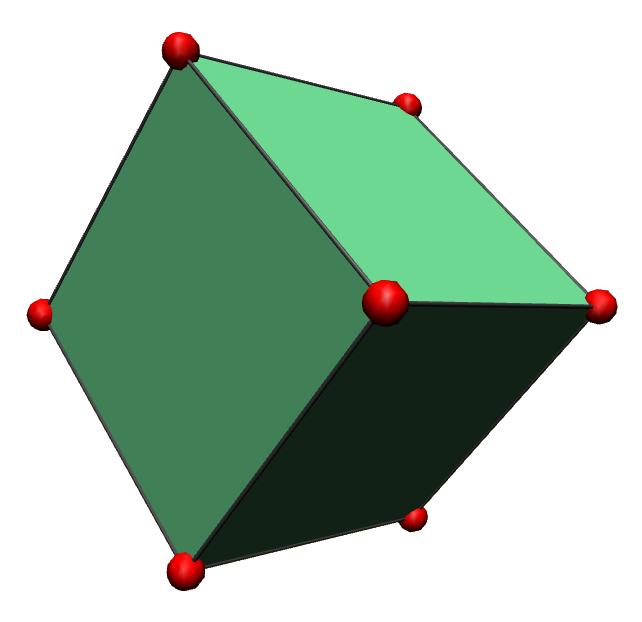
\includegraphics[width=.5\linewidth]{l6_cube.png}
  
  \caption{The representation of the cube in dimension 3 due with Polymake}
\label{fig:l6:1}
\end{figure}

To see a representation of graph of the polytope you can execute:

\texttt{polytope > \$p-> VISUAL\_FACE\_LATTICE;}

\begin{figure}[htbp]
  \centering
  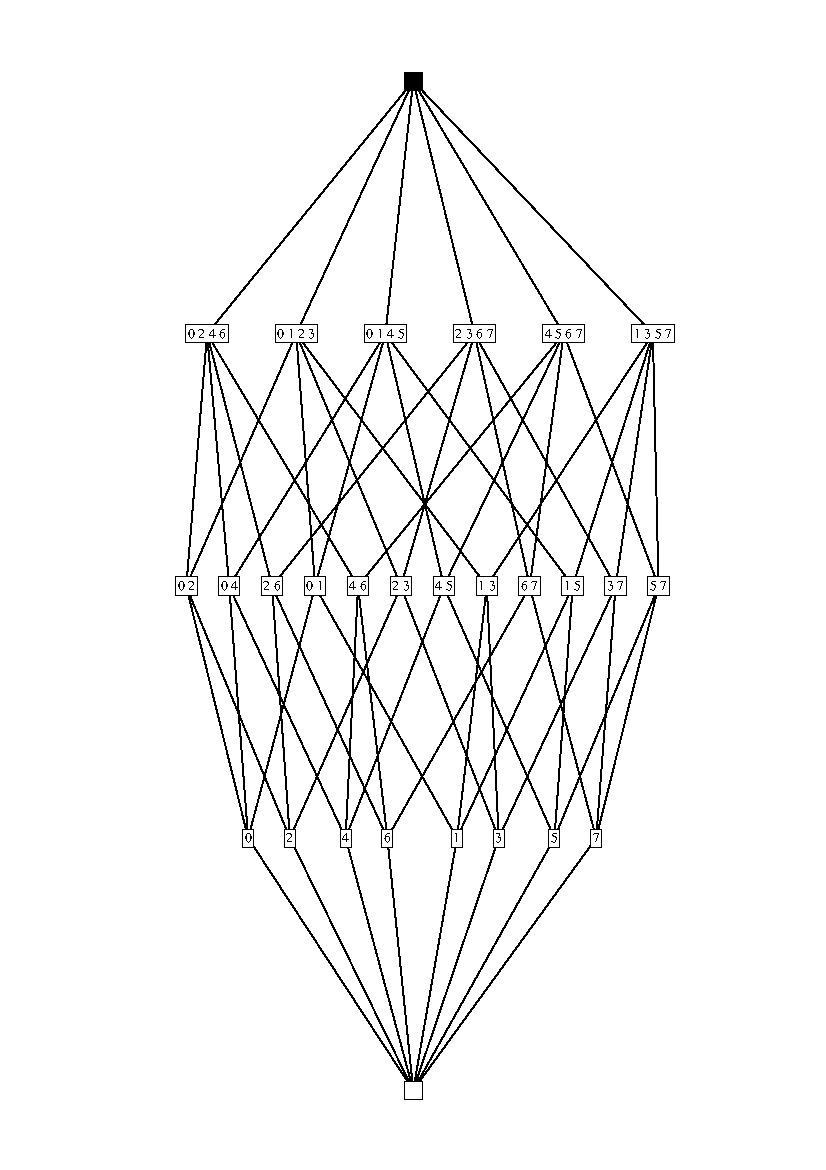
\includegraphics[width=0.9\linewidth]{l6_graph.jpg}
  
  \caption{The representation of the graph of the cube due with Polymake.}
\label{fig:l6:2}
\end{figure}

To see the equations of the facets you can type:

\texttt{polytope > print \$p->FACETS;}

\texttt{1 1 0 0}

\texttt{1 -1 0 0}

\texttt{1 0 1 0}

\texttt{1 0 -1 0}

\texttt{1 0 0 1}

\texttt{1 0 0 -1}

You must interpret as the following:

If you take $(1:1:0:0)$ gives you the facet: 

$$\left\langle(1:1:0:0)\left(\begin{array}{c}
                                                                     1\\	x\\	y\\	z
\end{array}\right)\right\rangle\geqslant 0$$

equivalently: $1+x\geqslant 0$ or $x\geqslant -1$. If you take $(1:-1:0:0)$ gives you the facet: $1-x\geqslant 0$ or $1\geqslant x$.
\newpage
We can polarize a polytope, for example:

\texttt{polytope > \$q=polarize(\$p);}

doing this, if we want to print the vertices of this new polytope, as we expected, gives the facets of the cube:

\texttt{polytope > print \$q->VERTICES;}

\texttt{1 -1 0 0}

\texttt{1 1 0 0}

\texttt{1 0 -1 0}

\texttt{1 0 1 0}

\texttt{1 0 0 -1}

\texttt{1 0 0 1}

Another thing that we can do is make Voronoi Diagrams. For example if we want to know the Voronoi Diagram of the points $(1,1),(0,1),(-1,1),(1,-1),(0,-1)\text{ and }(-1,-1)$:

\texttt{\$VD = new VoronoiDiagram(SITES=>[[1,1,1],[1,0,1],[1,-1,1],}

\texttt{[1,1,-1],[1,0,-1],[1,-1,-1]]);}

If we want to see a graphical representation:

\texttt{\$VD->VISUAL\_VORONOI;}

\begin{figure}[htbp]
  \centering
  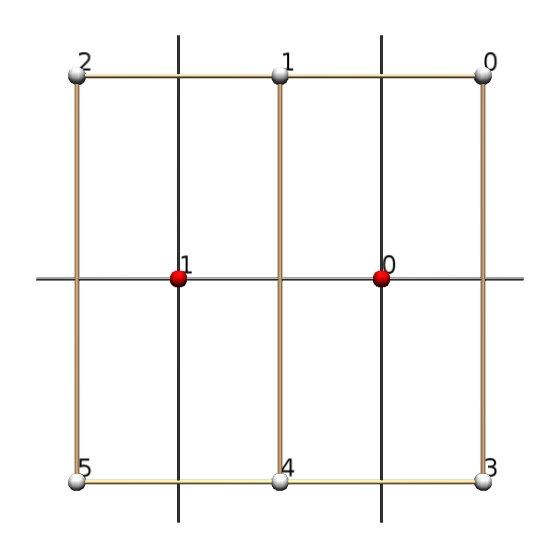
\includegraphics[width=0.7\linewidth]{l6_Voronoi.jpg}
  
  \caption{The representation of one Voronoi Diagram with Polymake.}
\label{fig:l6:3}
\end{figure}
\newpage
Other properties are, for example the facets equation:

\texttt{polytope > print \$VD->FACETS;}

\texttt{2 -2 -2 1}

\texttt{1 0 -2 1}

\texttt{2 2 -2 1}

\texttt{2 -2 2 1}

\texttt{1 0 2 1}

\texttt{2 2 2 1}

\texttt{1 0 0 0}

or the vertices of the diagram:

\texttt{polytope > print \$VD->VERTICES;}

\texttt{0 0 1 2}

\texttt{0 1 0 2}

\texttt{1 1/2 0 -1}

\texttt{0 -1 0 2}

\texttt{0 0 -1 2}

\texttt{1 -1/2 0 -1}

\section{Voronoi Cells in lattices}

Given a lattice $L\subset\RR^d$, find the facets of $$\Vor(0)=\{x\in\RR^d:\|x-0\|^2\leqslant\|x-v\|^2,\forall v\in L\}$$ 

\begin{defn}
 $v\in L$ is \textit{relevant} if the bisector of $v$ and $0$ contains a full dimensional face (i.e. a facet) of $\Vor(0)$.
\end{defn}

In $\ZZ^3$ we have a cube and the polytope defined by the relevant points is an octahedron.

\begin{obs}
 If the relevant vectors are precisely the minimal vector then $\Vor(0)$ is polar dual to the vertex figure of $0$ in $L$.
\end{obs}

\begin{theorem}[Georges Voronoi, 1908]
 A non-zero vector $v\in L$ is relevant if and only if $\pm v$ are the only shortest vectors in the coset $v+2L$.
\end{theorem}

\begin{proof}
 \underline{$\Longrightarrow$}

Suppose that $v,w\in L$ satisfy 

\begin{equation}\label{l6:eq1}
w\in v+2L 
\end{equation}

but

\begin{equation}\label{l6:eq2}
 w\neq \pm v
\end{equation}

and

\begin{equation}\label{l6:eq3}
 \langle w,w\rangle\leqslant \langle v,v\rangle
\end{equation}

Set:

\begin{center}
 $t=\frac{1}{2}(v+w)$ and  $u=\frac{1}{2}(v-w)$
\end{center}

Using (\ref{l6:eq1}) we have that $t,u\neq 0$ and using (\ref{l6:eq2}), $t,u\in L$. We have:

$$H_v=\{x\in\RR^d:\langle x,v\rangle\leqslant \frac{1}{2}\langle v,v\rangle\}$$

Let $x\in H_t\cap H_u$. Then:

$$\langle x,t\rangle\leqslant \frac{1}{2}\langle t,t\rangle$$ 

and

$$\langle x,u\rangle\leqslant \frac{1}{2}\langle u,u\rangle$$

Adding, we have:

$$\begin{array}{rcl}
   \langle x,v\rangle	&\leqslant	&\frac{1}{8}\left(\langle v,v\rangle+\langle w,w\rangle+2\langle v,w\rangle+\langle 							v,v\rangle+\langle w,w\rangle-\langle v,w\rangle\right)\\
			&=		&\frac{1}{4}\left(\langle v,v\rangle+\langle w,w\rangle\right)\\
			&\leqslant	&\frac{1}{2}\langle v,v\rangle
  \end{array}
$$ 

Were in the last one we have used (\ref{l6:eq3}). So $x\in H_v$, therefore $v$ is not relevant.

 \underline{$\Longleftarrow$}
Suppose $v\in L$ is not relevant. Then there exists some $w \in L$. $w\neq 0$, $w\neq \pm v$ with:

\begin{equation}\label{l6:eq4}
 \left\langle \frac{1}{2} v, w\right\rangle \geqslant \frac{1}{2}\langle w,w\rangle
\end{equation}

and $\frac{1}{2}v\notin H_w$.Then

$$\begin{array}{rcl}
   \|v-2w\|^2 	&=		&\langle v-2w,v-2w\rangle \\
		&=		&\langle v,v\rangle - 4 \langle v,w\rangle + 4 \langle w,w\rangle\\
		&\leqslant	&\langle v,v\rangle - 4 \langle v,w\rangle + 4 \langle v,w\rangle\\
		&=		&\langle v,v\rangle
  \end{array}
$$

where in the inequality we have used (\ref{l6:eq4}), and is in $v+2L$, not $0$, $w\in L$.

\end{proof}

% Local Variables: 
% mode: latex
% TeX-master: "dag-upc"
% End: 




\chapter{Lattice Geometry}

\scribe{Borja Elizale}

A $\mathbb{Z}$-module is an abelian group of rank $r$, and we don't care about the torsion part, so it is isomorphic to $\mathbb{Z}^r$ for some $r$.
\begin{defn}
A lattice polytope is a convex polytope all whose vertices have integral coordinates.
\end{defn}
A natural question that can arise is how can we know if the two lattice polytopes are equivalent. The answer to this question is that they are equivalent when they are related by an invertible mapping that leaves the lattice invariant. These mappings belong to the set of mappings:
\begin{center}
Isom$(\mathbb{Z}^d)$=$Sl_d(\mathbb{Z})\times$ Translations$(\mathbb{Z})$
\end{center}
And $Sl_d(\mathbb{Z})$ are the $d\times d$ matrices over the integer numbers that have determinant equal to 1 or -1.
Let's consider, as an example, the lattice polytopes in the plane:
\begin{equation}
P_1=conv(\{0,e_1,e_2\})
\end{equation}
\begin{equation}
P_2=conv(\{0,e_1,7e_1+e_2\})
\end{equation}
\begin{equation}
P_3=conv(\{0,e_1,7e_1+2e_2\})
\end{equation}
We want to know if they are equivalent or not, and based on what we have said before, this happens if there exists a transformation in $Sl_d(\mathbb{Z})$ (in this case the dimension is 2) plus a translation that brings one to the other. Since the two first points are the same for the three polytopes, there is no translation and so we only have to find a transformation in $SL_d(\mathbb{Z})$ between them.
Now for the first one this is equivalent to find a matrix $\mathbf{A}$ such that:
\begin{equation}
\mathbf{A}\left[\begin{matrix}1&0\\0&1\end{matrix}\right]=\left[\begin{matrix}1&7\\0&1\end{matrix}\right]
\end{equation}
And clearly $\mathbf{A}$ must be the matrix from the right side of the equation, which is in the set $SL_d(\mathbb{Z})$.
For the second case this does not happen, the right side of the equation will be the matrix $\left[\begin{matrix}1&7\\0&2\end{matrix}\right]$, which is not in $SL_d(\mathbb{Z})$. So such a transformation does not exist and they are not equivalent.
Computing the volume of a lattice polytope is computing the determinant of the square matrix built from the homogeneous coordinates of the points. This doesn't give properly the volume, but the volume of the smallest parallelepiped that contains the whole polytope.
We say that a lattice simplex, $\Delta$ is:

\begin{defn}
\emph{Unimodular} if $\det\Delta=\pm 1$
\end{defn}
\begin{defn}
\emph{Empty} if conv$\Delta\cap\mathbb{Z}^d=$vertices of $\Delta$.
\end{defn}
\begin{defn}
\emph{Standart} if $\Delta$ is equivalent to conv$\{0,e_1,...,e_d\}$
\end{defn}
The relation between these concepts goes as follows:
\begin{center}
\textbf{Standart}$\Leftrightarrow$\textbf{Unimodular}$\Rightarrow$ \textbf{Empty}
\end{center}
And if the dimension is equal to 2 we also have
\begin{center}
\textbf{Empty}$\Rightarrow$\textbf{Unimodular}
\end{center}
But the other implication is not true in general (there is a counter example for dimension 3, and then for every dimension larger than 3).
Let's proof the first relationship
\begin{proof}
$\Delta$ Standart $\Rightarrow$ Unimodular. If $\Delta$ is such that $\mathbf{A}\Delta=\mathbf{A}_0$, for some $\mathbf{A}$ in $SL_d(\mathbb{Z})$, then it happens that $\det(\mathbf{A}\Delta)=\det(\mathbf{A}_0)$, and then $\pm 1\det(\Delta)=\pm1$ and this only happens if $\det(\Delta)=\pm1$, which is the condition for it to be unimodular.

For the reciprocal, if $\Delta$ is unimodular, then $\det(\Delta)=\pm 1$, and if we want some $\mathbf{A}$ in $SL_d(\mathbb{Z})$ that satisfies $\mathbf{A}\Delta=\mathbf{A}_0=Id(d)$, then $\mathbf{A}=\Delta^{-1}$ and $\Delta^{-1}$ belongs to $SL_d(\mathbb{Z})$ because it's determinant is $\pm 1$.
\end{proof}
\begin{proof}
\textbf{Unimodular} $\Rightarrow$ \textbf{Empty}. By contradiction, if it was not empty, then we could divide the polytope into two subdivisions by taking the cones to the interior point that makes it non empty, so that each subdivision has area, at least, $\pm 1$ and then whole area (which is the sum of the parts) would be greater than $1$ contradicting the unimodularity.
\end{proof}
\begin{thm}
Pick's theorem: if $P\subset\mathbb{R}^2$ is a reticular polygon, then area($P)=I+\frac{B}{2}-1$. Where $I=$ Int$P\cap\mathbb{Z}^2$ and $B=\partial P\cap\mathbb{Z}^2$.
\end{thm}

This theorem allows us to prove that for $d=2$, \textbf{Empty}$\Rightarrow$\textbf{Unimodular}, because if it is empty, then $I=0$ and then $\frac{A}{2}=0+\frac{3}{2}-1$ and $A=1$ so the polygon it is unimodular as well.


\end{document}

\chapter{Ehrhart-Macdonald Reciprocity}

\scribe{Albert Santiago}

\section{Statement of the theorem}

Let $P$ be a lattice polytope. Let $L_P:\NN\longrightarrow\NN$ be the lattice point counting function,
\[\begin{array}{cccl}
  L_P: &\NN &\longrightarrow &\NN \\
  &t &\longmapsto &L_P(t)=\#\left\{tP\cap\ZZ^d\right\}
\end{array}\]

and let $L_{P^0}:\NN\longrightarrow\NN$ be the lattice point counting function in the interior of $P$.

By Ehrhart's Theorem seen in the previous lecture, it is known that $L_P, L_{P^0}\in\QQ[t]$.

\begin{theorem}[Ehrhart-Macdonald Reciprocity]
\[
  L_P(-t) = (-1)^d L_{P^0}(t)
\]
\end{theorem}

Note that in previous lecture we have already seen an example for this EM reciprocity for the cube. Indeed,
\begin{align*}
  L_{\Box^d}(t) &= (1+t)^d\\
  L_{(\Box^d)^0}(t) &= (-1)^d(1-t)^d
\end{align*}

\bigskip
\section{Auxiliary results}

\begin{proposition}
  Let $w_1,\ldots,w_d\in\ZZ^d$ be linearly independent. Let $C=\cone{w_1,\ldots,w_d}$ be cone over a simplex. Let $v\in\RR^d$ such that $\partial(v+C)\cap \ZZ^d=\varnothing$. Then,
  \[
    \sigma_{v+C}\left(\frac{1}{z_1},\cdots,\frac{1}{z_d}\right) = (-1)^d \sigma_{-v+C}(z_1,\ldots,z_d)
  \]
\end{proposition}

\emph{Notes}:
\begin{itemize}
 \item For the existence of such $v\in\RR^d$, see exercise sheet \#6.
 \item $\sigma_{v+C}\left(\frac{1}{z_1},\cdots,\frac{1}{z_d}\right)$ is not a power series, so the theorem is meaningless at this level. At most, we can say it is an element from $\QQ[z_1,\ldots,z_d]$, where the theorem holds.
 \item Try to see $\frac{1}{z_i}$ as the variables corresponding to $-P$.
\end{itemize}

\begin{proof}
  To be done. %TODO
\end{proof}

\begin{proposition}[Stanley Reciprocity]
  Let $C$ be a rational pointed cone (i. e. $C=\cone{w_1,\ldots,w_d}, w_i\in\QQ^d$) with apex at the origin. Then,
  \[
    \sigma_C\left(\frac{1}{z}\right)=(-1)^d\sigma_{C^0}(z)
  \]
\end{proposition}

\begin{proof}
  To be done. %TODO
\end{proof}

\begin{definition}
  We define the Ehrhart function for the interior lattice points of a polytope naturally as
  \[
    \Ehr_{P^0}(z):=\sum_{t\geq 1} L_{P^0}(t)z^t
  \]
\end{definition}

\emph{Note}: We can start the sum at $t=1$ rather than at $t=0$ because the origin is not an interior point of $P$.

\begin{observation}
  As it happened with the original Ehrhart function, the following equality holds:
  \[
    \Ehr_{P^0}(z)=\sigma_{\cone(P^0)}(1,\ldots,1,z)
  \]
\end{observation}

\begin{proposition}
  Let $P$ be a lattice polytope. Then,
  \[
    \Ehr_(P^0)(z)=(-1)^{\dim{P}+1} \Ehr_P\left(\frac{1}{z}\right)
  \]
\end{proposition}

\emph{Notes}:
\begin{itemize}
 \item The proposition is also valid for $P$ any \emph{rational} polytope, not only for lattice polytopes.
 \item Not every polytope can be perturbed into a rational one. There exist irrational polytopes.
\end{itemize}

\begin{proof}
  To be done. %TODO
\end{proof}

\bigskip
\section{Proof of Ehrhart-Macdonald Reciprocity}
To be done. %TODO

\bigskip
\section{Degree of a lattice polytope}

\begin{observation}
  Let $p\in\QQ[t]$ be a polynomial of degree $d$. If the following equality holds:
  \[
    \sum_{t\geq 0}p(t)z^t = \frac{h_dz^d+\cdots h_1z+h_0}{(1-z)^d}
  \]
  then
  \[
    \left.\begin{array}{r}
	     h_d=\cdots=h_{k+1}=0\\
	     h_k\neq0
          \end{array}\right\}
    \Longleftrightarrow
    \left\{\begin{array}{l}
             p(-1)=p(-2)=\cdots=p(-(d-k))=0\\
             p(-(d-k+1))\neq0
           \end{array}\right.
  \]
\end{observation}

\begin{proof}
  See Theorem 3.18 at Beck-Robins' \emph{Computing the continuous discretely}.
\end{proof}

\begin{proposition}
  Let $P\subset\RR^d$ be a lattice polytope with Ehrhart function:
  \[
    \Ehr_P(z) = \frac{h_dz^d+\cdots h_1z+h_0}{(1-z)^d}
  \]
  Then,
  \[
    \left.\begin{array}{r}
	     h_d=\cdots=h_{k+1}=0\\
	     h_k\neq0
          \end{array}\right\}
    \Longleftrightarrow
    \left\{\begin{array}{l}
             L_P(-1)=L_P(-2)=\cdots=L_P(-(d-k))=0\\
             L_P(-(d-k+1))\neq0
           \end{array}\right.
  \]
\end{proposition}

\begin{definition}
  We call $k$ the \emph{degree of the lattice polytope $P$}.
\end{definition}

\begin{observation}
  If $P$ is a $d$-polytope of degree $k$, then $L_P(-(d-k))=(-1)^d L_{P^0}(-(d-k))=0$, so the $(d-k)$-th dilate of $P$ does not contain any interior lattice point, and $(d-k+1)P$ is the smallest integer dilate that contains an interior lattice point.
\end{observation}

%TODO examples?


\bigskip 
\section{Reflexive polytopes}
\begin{definition}
  A lattice polytope $P$ with $0\in P$ is \emph{reflexive} if $P$ can be expressed as:
  \[
    P=\{x\in\RR^d:Ax\leq\mathbbm{1}\}
  \]
  where $A\in\ZZ^{n\times d}$ is an integer matrix.
\end{definition}

\begin{observation}
  To be done. %TODO
\end{observation}

To be ended. %TODO







\chapter{Systems of sparse polynomial equations}

\scribe{Anna Somoza}
 
\textbf{Goal:} Our aim is to construct systems of sparse polynomial equations with non-trivial lower-bound on the number of real solutions.

\textbf{Motivation:} We think abount this problem inspired by Kouchironko bound: Given the polynomial system
$$\begin{cases}
F_1(x_1,\dots,x_n) = 0\\
\vdots\\
F_n(x_1,\dots,x_n) = 0\\
\end{cases}$$

such that they share the same Newton polynomial $N(F_i)$, then we get that the number of complex solutions for the system is $\operatorname{vol} N(F_i)$.


\textbf{Tools:} We will introduce:
\begin{enumerate}
\item A generalization of Veronese embedding,
\item replace system of polynomial equations in
$$(\CC^*)^n = \CC^n \backslash \{\bigcup_i\{x_i = 0\}\}$$
by a system of linear equations in $\mathbb{P}^{\Delta \cap \ZZ^n} = \mathbb{P}^\Delta$:
\begin{align*}
\varphi_\Delta : (\CC^*)^n  &\to \mathbb{P}^\Delta\\
(t_1,\dots,t_n) &\mapsto [t^m : m\in \Delta \cap \ZZ^n]
\end{align*}
\end{enumerate}

\begin{example}
For $n = 1$
\begin{align*}
\varphi_\Delta : \CC^*  &\to \mathbb{P}^\Delta\\
t &\mapsto [1:t:t^2:t^3]
\end{align*}
\end{example}

- Degree of a map between orientable mainfolds:

$X_\Delta = \operatorname{cl}(\Im \varphi_\Delta)$ in a Zariski topology

toric ($(\CC^*)^n$ acts on $X_\Delta$) variety associated to $\Delta$.



\section{Wronski polynomials}

We require a foldable (i.e. rainbow colored), full and regular triangulation of $L$.

\begin{definition}
A triangulation $T$ is said to be foldable if there exists a graph homomorphism such that
$$\operatorname{sk}^1(T) = \operatorname{sk}^1(\conv\{0,e_1,\dots,e_n\}).$$

It is equivalent to say that it is foldable if and only if its dual graph is bipartite.
\end{definition}

\begin{figure}
\begin{tikzpicture}
\draw (0,0) -- (1,0) -- (2,1) -- (2,2) -- (1,2) -- (0,1) -- cycle;
\draw[red, dashed] (0,0) -- (1,1);
\draw[red, dashed] (0,1) -- (1,1);
\draw[red, dashed] (1,0) -- (1,1);
\draw[red, dashed] (1,2) -- (1,1);
\draw[red, dashed] (2,1) -- (1,1);
\draw[red, dashed] (1,2) -- (2,1);
\end{tikzpicture}
\caption{A non-foldable triangulation}
\end{figure}

\begin{figure}
\begin{tikzpicture}
\draw (0,0) -- (1,0) -- (2,1) -- (2,2) -- (1,2) -- (0,1) -- cycle;
\draw[red, dashed] (0,1) -- (1,0);
\draw[red, dashed] (0,1) -- (1,1);
\draw[red, dashed] (1,0) -- (1,1);
\draw[red, dashed] (1,2) -- (1,1);
\draw[red, dashed] (2,1) -- (1,1);
\draw[red, dashed] (1,2) -- (2,1);
\end{tikzpicture}
\caption{A non-foldable triangulation}
\end{figure}


\begin{definition}
We say that a triangulation is full if and only if
$$\operatorname{sk}^0 T = \Delta \cap \ZZ.$$
\end{definition}

\begin{definition}
We say that a triangulation is regular if and only if it is induced by a convex height function on $\Delta \cap \ZZ^n$
\end{definition}
% Local Variables: 
% mode: pdflatex
% TeX-master: "dag-upc"
% End: 

\chapter*{Scribes 2013}

\section{Alex Alvarez}
I have done a double degree in Informatics Engineering and Mathematics at the UPC and during these years I have participated in programming contests both individually and representing the UPC. I am mainly interested in Algorithms and Data Structures and I would like to start a PhD in those topics next year, but I also enjoy learning about Discrete Mathematics, in particular Combinatorics and Graph Theory.


\section{Cecilia Gir\'on Albert}

I've got my Degree in Mathematics at the Universidad Aut\'onoma de Madrid, which I completed my fifth and sixth semesters 
at the University of Jyv\"askyla (Finland) as an Erasmus student. My degree has been mainly focused on subjects like 
analysis, statistics and numerical methods, although I am more interested in algebra and graph theory. 

I decided to study the Master in Advanced Mathematics and Mathematical Engineering to keep developing my mathematics skills 
in some theoretical subjects that can be applied in real life problems. Therefore, I believe that this course is a great 
opportunity to learn more about algorithmic and computing science and even more importantly, it may help me to find out 
what field I would like to focus on in the future.

\section{Anna Somoza}

I have recently finished a degree in Mathematics at the Universitat Polit\`ecnica de Catalunya. During this degree I developed a great interest in Algebra fields. In particular, I took the optional subjects \emph{Algebraic Geometry}, \emph{Algebraic Topology} and \emph{Galois Theory} and I wrote my Final Degree Thesis on a topic of Number Theory.

Now I'm taking the Master in Advanced Mathematics and Mathematical Engineering to develop my knowledge in these and other fields, and I my aim is to start a PhD in Number Theory next year. I enroled this subject because I have allways liked both computer science and geometry, and it seemed to be interesting. Therefore, I would be interested in the topic related to algebraic geometry.

\section{Daniel Torres}

My name is Daniel Torres and I am graduate in mathematics in UPC. Along the degree I have developed much interest in fields of topology, algebra and geometry, and some loathing to study (not to programming) numerical methods and modelling. I decided study this master, and particularly this subject, for expand my knowledge about my interests.

More concretely, I am doing this course with the hope it shows me about geometry.




% Local Variables: 
% mode: latex
% TeX-master: "dag-upc"
% End: 



\bibliographystyle{plainnat}
\bibliography{dag}

\renewcommand{\chaptername}{Chapter}
\chapter*{Papers to referee}


\bibliographystyle{amsplain}
\bibliography{papers-to-referee}

\nocite{donoho}
\nocite{eppstein-ziegler-fat-4-polytopes}
\nocite{friedman-graph-simple-polytope}
\nocite{gebert-sturmfels-theobald}
\nocite{haase-schicho}
\nocite{sanyal}
\nocite{schwartz-ziegler}
\nocite{sottile}
\nocite{szabo-welzl}
\nocite{welzl}

% Local Variables: 
% mode: latex
% TeX-master: "dag-upc"
% End: 


\end{document}

%%% Local Variables: 
%%% mode: latex
%%% TeX-master: t
%%% End: 
